\documentclass[]{acmsiggraph}
\usepackage{algorithm}
\usepackage[noend]{algpseudocode}
\TOGonlineid{45678}
\TOGvolume{0}
\TOGnumber{0}
\TOGarticleDOI{0}
\TOGprojectURL{}
\TOGvideoURL{}
\TOGdataURL{}
\TOGcodeURL{}
\usepackage{color}
%\definecolor{red}{rgb}{0.9, 0.17, 0.31}
\usepackage{multirow}
\usepackage{subfig}
\usepackage{xcolor}
\usepackage{lipsum}
\usepackage{listings}
\usepackage{graphicx}
\usepackage{glsllst} % My own package providing markup listing for glsl
\usepackage{rmlst}   % My own package providing markup listing for renderman
\usepackage{amsmath}
\usepackage{hyperref}

\lstset{
	backgroundcolor=\color[rgb]{0.95, 0.95, 0.95},
	tabsize=3,
	%rulecolor=,
	basicstyle=\footnotesize\ttfamily,
	upquote=true,
	aboveskip={1.5\baselineskip},
	columns=fixed,
	showstringspaces=false,
	extendedchars=true,
	breaklines=true,
	prebreak = \raisebox{0ex}[0ex][0ex]{\ensuremath{\hookleftarrow}},
	frame=none,
	aboveskip=15pt,
	belowskip=8pt,
	captionpos=t,
	showtabs=false,
	showspaces=false,
	showstringspaces=false,
	identifierstyle=\ttfamily,
	%keywordstyle=\color{red}\bfseries,
	%keywordstyle=[1]\bfseries\color{syntaxBlue},
	%keywordstyle=[2]\bfseries\color{syntaxRed},
	%keywordstyle=[3]\color{blue}\bfseries,
	%keywordstyle=[4]\bfseries\color{syntaxBlue},
	commentstyle=\color[rgb]{0.082,0.639,0.082},
	keywordstyle=[1]\bfseries\color[rgb]{0,0,0.75},
	keywordstyle=[2]\bfseries\color[rgb]{0.5,0.0,0.0},
	keywordstyle=[3]\bfseries\color[rgb]{0.127,0.427,0.514},
	keywordstyle=[4]\bfseries\color[rgb]{0.4,0.4,0.4},
	stringstyle=\color[rgb]{0.639,0.082,0.082},
}

\title{ECG Heartbeat Classification Using Machine Learning Applications}

\author{Anh Quan Nguyen BI12-365\thanks{e-mail: quanna.bi12-365@st.usth.edu.vn}\\University of Science and Technology of Hanoi}
\pdfauthor{Anh Quan Nguyen}

\keywords{rendering}

\begin{document}

\maketitle


\begin{abstract}
ECG heartbeat signals, extracted from electrocardiograms, offer vital information about the heart's electrical activity. Analyzing these signals is crucial for identifying abnormalities like arrhythmias or myocardial infarctions, and facilitating early intervention in cardiac conditions. Employing machine learning and deep learning models for ECG signal classification is a strategic approach to improve the efficiency and precision of heart-related issue diagnoses. This practical application holds promise for transforming cardiovascular healthcare by enabling timely and accurate interventions, ultimately elevating patient outcomes and alleviating the strain on healthcare systems.
\end{abstract}
%\keywordlist
%\TOGlinkslist

\section{Introduction}

\subsection{Context and Motivation}
Cardiovascular diseases remain a leading cause of global morbidity and mortality, emphasizing the critical need for advancements in diagnostic methodologies. In this context, the analysis of electrocardiogram (ECG) heartbeat signals emerges as a pivotal tool for the early detection of cardiac irregularities such as arrhythmias and myocardial infarctions. The significance of precise ECG signal classification lies in its potential to revolutionize cardiovascular healthcare by enabling timely interventions and improving patient outcomes.

\subsection{Objectives}
The primary objective of this study is to explore the application of machine learning models, specifically decision tree and convolutional neural network (CNN) architectures, in enhancing the accuracy and efficiency of ECG signal classification. Through this exploration, we aim to provide valuable insights into the interpretability and feature importance of decision tree models, while leveraging the intricate pattern recognition capabilities of CNN architectures. These objectives align with the broader goal of advancing diagnostic tools and methodologies for cardiac health monitoring.

\subsection{Related Works}
Prior research has significantly shaped the landscape of ECG signal analysis. Notably, Hassaballah et al. \cite{hassaballah2023} implemented machine learning in developing Smart Healthcare Systems, providing insights into transfer learning. Additionally, Mohammad Kachuee et al. made noteworthy contributions in classifying using residential networks \cite{kachuee2018}. These influential works not only inform our study but also highlight the evolving nature of ECG signal analysis, guiding our research within this dynamic field.

\section{Dataset Understanding}
The dataset utilized in this study is sourced from real-world ECG signals, specifically obtained from the MIT-BIH Arrhythmia Dataset. This collection comprises 109,446 heartbeat signals, each preprocessed and segmented to represent distinct cardiac events. The dataset encompasses a variety of cardiac conditions, offering a comprehensive representation of the electrocardiogram (ECG) patterns associated with different arrhythmias and myocardial infarctions.

The dataset is categorized into five primary classes, each corresponding to a specific cardiac event type:

\textbf{N (Normal):}
\begin{itemize}
    \item Normal heartbeats without any abnormalities.
\end{itemize}

\textbf{S (Supraventricular):}
\begin{itemize}
    \item Atrial premature beats, aberrant atrial premature beats, nodal premature beats, and supra-ventricular premature beats.
\end{itemize}

\textbf{V (Ventricular):}
\begin{itemize}
    \item Premature ventricular contractions, ventricular escape beats.
\end{itemize}

\textbf{F (Fusion):}
\begin{itemize}
    \item Fusion of ventricular and normal beats.
\end{itemize}

\textbf{Q (Unclassifiable):}
\begin{itemize}
    \item Paced beats, fusion of paced and normal beats, and beats that are unclassifiable.
\end{itemize}

This dataset meticulously categorizes various cardiac events, enabling a deeper dive into ECG signal classification. Grasping these categories is crucial for both training and evaluating machine learning models, as the range of conditions reflects the complexities of real-world cardiac scenarios. This detailed description of the dataset serves as the foundation for our subsequent analyses and classification tasks, ultimately aiming to improve the accuracy and expand the reach of ECG heartbeat classification in smart healthcare systems.

The dataset is provided in CSV file format, with separate training and testing sets, each contains 187 features with the last one represents the labels, the output of the project, making it simpler for us to manipulate and implement numerous approaches and operations. 
\section{Method}
\subsection{Data Preprocessing}
The dataset seems to be imbalanced with the majority of elements in the Normal class, this can provide various negative effects on the classification results as this problem makes the model perform poorly on the minority classes, misleading the metrics and bringing about serious consequences in medical diagnosis.

\begin{figure}[h]\centering
 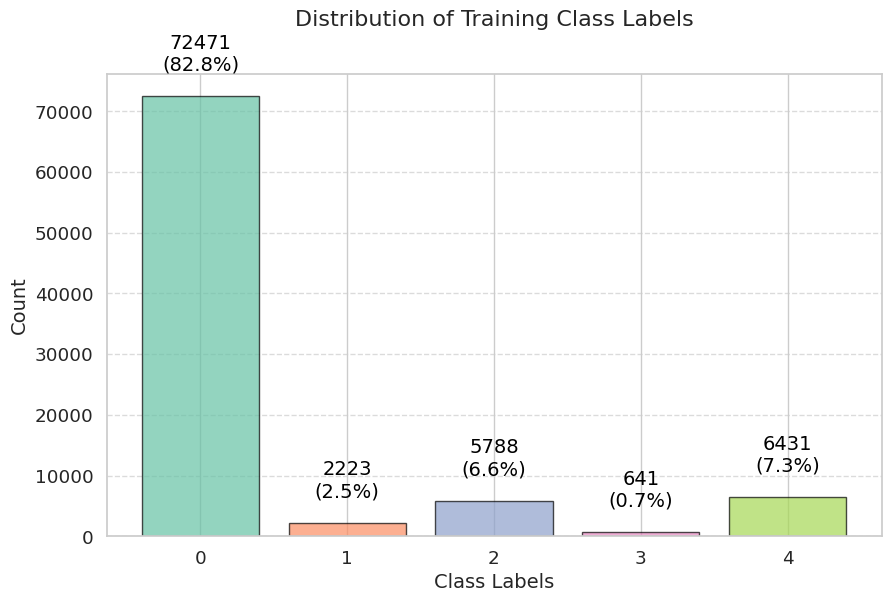
\includegraphics[width=0.75\linewidth]{images/dis_class.png}
 \caption{\label{fig:reference}The distribution of instances of each class.}
\end{figure}

Therefore, to mitigate this imbalance and enhance the model's ability to accurately classify diverse events, we employ the Synthetic Minority Over-sampling Technique (SMOTE) during the preprocessing stage. SMOTE is an upsampling technique that generates synthetic instances for the minority classes by identifying similar data points within this class, slightly adjusting their features, and creating new data points based on these adjustments, effectively balancing the representation of all classes.

\begin{figure}[h]\centering
 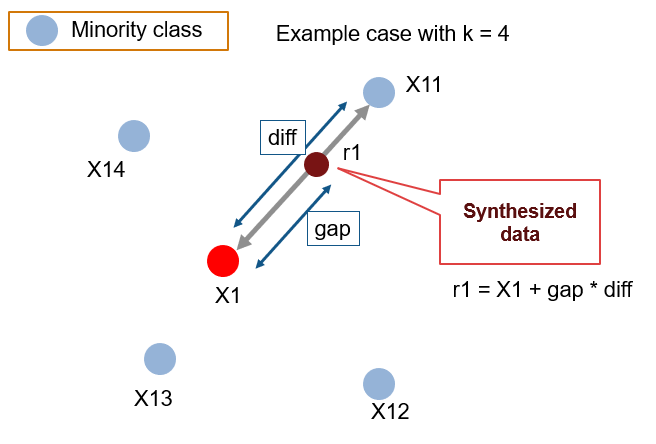
\includegraphics[width=0.75\linewidth]{images/smote.png}
 \caption{\label{fig:reference}SMOTE operation .}
\end{figure}

We applied this method to resample the training dataset, resulting in a new larger dataset with an equal amount of occurrences in all categories.

\begin{figure}[h]\centering
 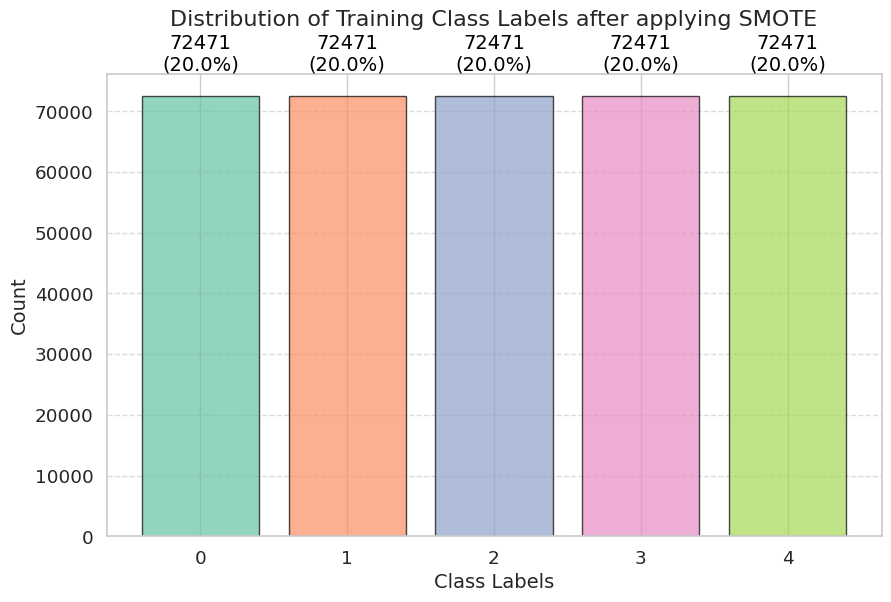
\includegraphics[width=0.75\linewidth]{images/dis_class_smote.png}
 \caption{\label{fig:reference}The distribution of instances of each class after applying SMOTE.}
\end{figure}

\subsection{Dataset splitting}
As mentioned above, the dataset contains 2 distinguished sets for training and testing. 
We only split the resampled training set into 2 train-valid sets (with ratio 8-2) in the deep learning approach because of its higher parameter count and increased risk of overfitting, benefit from an additional validation set will optimize hyperparameters and enhance generalization to new data, while machine learning model tends to be lower in parameters complexity.

\subsection{Machine Learning Approach}
The resampled data is fitted into a Decision Tree model which consists of Gini impurity split measurement, two minimum number of samples to split an internal node and one minimum sample to be at a leaf node. The Decision Tree's interpretability, inherent ability to handle diverse data types, and efficient management of missing values make it a compelling choice for this analysis, facilitating clear understanding of dataset's characteristics

\subsection{Deep Learning Approach}
In this approach, we build and implemented a Convolutional Neural Network (CNN) with the input sequence of length 187 and a single channel, with 152965 trainable parameters and a total of 10 layers

\begin{figure}[h]\centering
 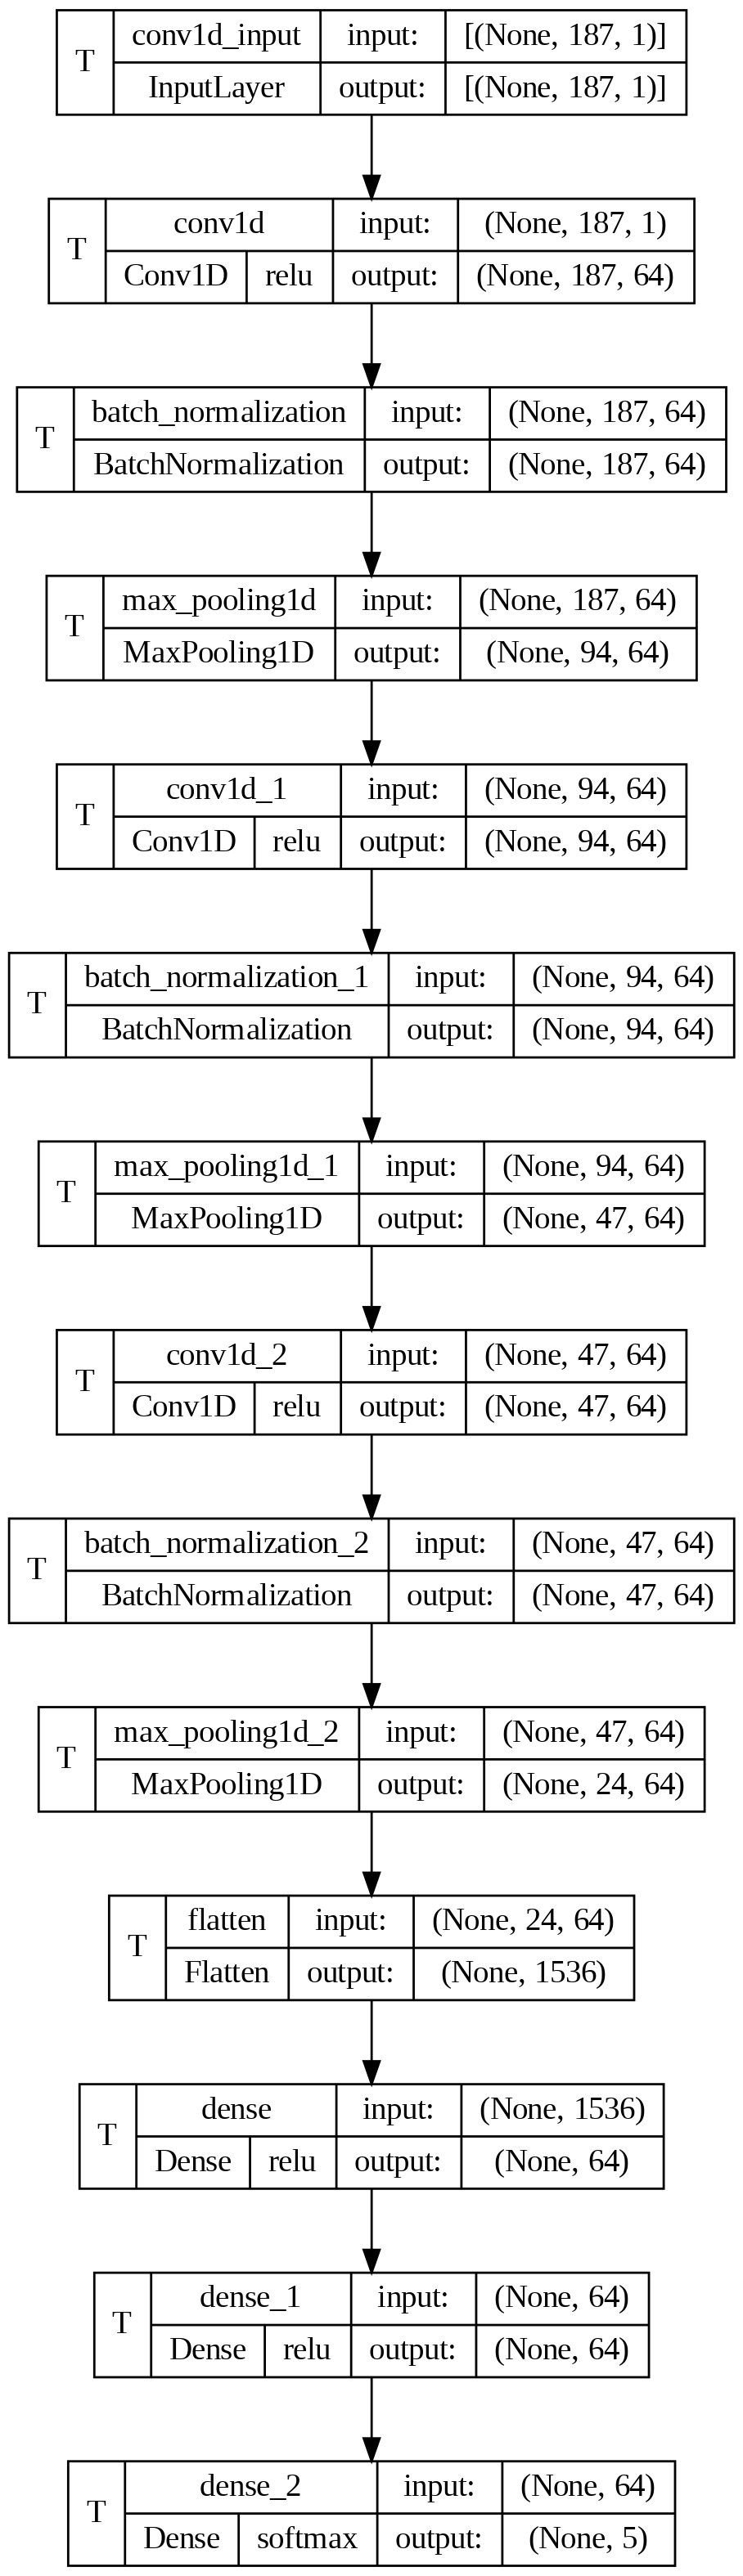
\includegraphics[width=0.5\linewidth]{images/cnn.png}
 \caption{\label{fig:reference}Deep learning model architecture.}
\end{figure}

The model includes three Convolutional 1-D layers, each followed by batch normalization and max pooling. Activation functions such as ReLU are employed to introduce non-linearity, enhancing the model's capacity to learn complex patterns. The output layer with a softmax activation function yields a probability distribution over five classes, aligning with the goal of classifying heartbeat signals into different categories.

\subsection{Losses and Metrics}

The CNN model employs categorical crossentropy loss (\(\mathcal{L}_{\text{CCE}}\)) for multiclass classification:

\[
\mathcal{L}_{\text{CCE}} = - \sum_{i=1}^{N} \sum_{j=1}^{C} y_{ij} \cdot \log(p_{ij})
\]

where \(N\) is instances, \(C\) is classes, \(y_{ij}\) is true class indicator, and \(p_{ij}\) is predicted probability.

For evaluation, various metrics are utilised to assess both Decision Tree and CNN models:

\textbf{Accuracy (\(\text{Acc}\)):}
\[
\text{Acc} = \frac{\text{Correct Predictions}}{\text{Total Predictions}}
\]

\textbf{Precision (\(\text{Prec}\)):}
\[
\text{Prec} = \frac{\text{True Positives}}{\text{True Positives + False Positives}}
\]

\textbf{Recall (\(\text{Rec}\)):}
\[
\text{Rec} = \frac{\text{True Positives}}{\text{True Positives + False Negatives}}
\]

\textbf{F1 Score (\(\text{F1}\)):}
\[
\text{F1} = 2 \cdot \frac{\text{Prec} \cdot \text{Rec}}{\text{Prec + Rec}}
\]
\section{Results} \label{sec:overview}

\subsection{Decision Tree Model}

\begin{center}
\begin{tabular}{lcccc}
\hline
\textbf{Class} & \textbf{Precision} & \textbf{Recall} & \textbf{F1-Score} & \textbf{Support} \\
\hline
Normal & 0.95 & 0.98 & 0.97 & 17539 \\
Supraventricular & 0.75 & 0.49 & 0.59 & 849 \\
Ventricular & 0.90 & 0.82 & 0.85 & 1596 \\
Fusion & 0.73 & 0.43 & 0.55 & 274 \\
Unclassifiable & 0.94 & 0.93 & 0.94 & 1634 \\
\hline
\textbf{Accuracy} & \multicolumn{4}{c}{0.94} \\
\textbf{Macro Avg} & \multicolumn{4}{c}{0.86 / 0.73 / 0.78} \\
\textbf{Weighted Avg} & \multicolumn{4}{c}{0.94 / 0.94 / 0.94} \\
\hline
\end{tabular}
\end{center}


\subsection{CNN Model}

\begin{center}
\begin{tabular}{lcccc}
\hline
\textbf{Class} & \textbf{Precision} & \textbf{Recall} & \textbf{F1-Score} & \textbf{Support} \\
\hline
Normal & 0.99 & 0.99 & 0.99 & 18062 \\
Supraventricular & 0.86 & 0.81 & 0.83 & 586 \\
Ventricular & 0.96 & 0.97 & 0.96 & 1435 \\
Fusion & 0.85 & 0.67 & 0.75 & 206 \\
Unclassifiable & 0.99 & 0.99 & 0.99 & 1603 \\
\hline
\textbf{Accuracy} & \multicolumn{4}{c}{0.98} \\
\textbf{Macro Avg} & \multicolumn{4}{c}{0.93 / 0.89 / 0.91} \\
\textbf{Weighted Avg} & \multicolumn{4}{c}{0.98 / 0.98 / 0.98} \\
\hline
\end{tabular}
\end{center}

It can be concluded that the SMOTE method handled class imbalanced dataset effectively as the results show nearly no classification bias.

Decision Tree model demonstrates strong precision and recall for the majority class (Normal), achieving an overall accuracy of 94\%. However, it exhibits lower performance on minority classes (Supraventricular, Fusion) with relatively lower precision and recall.

On the other hand, the CNN model showcases remarkable precision, recall, and F1-score across all classes, particularly excelling in correctly identifying minority classes. The overall accuracy of 98\% underscores the model's proficiency in discerning intricate patterns within ECG heartbeat signals. 

These results signify the efficacy of deep learning in enhancing the classification of diverse heartbeat patterns compared to traditional Decision Tree methods.

\section{Discussion}

\subsection{Drawbacks}

\paragraph{Imbalance Handling:}While the CNN model demonstrates overall effectiveness, addressing potential class imbalance issues is crucial, particularly for minority classes. Imbalanced datasets can introduce bias and impact the accuracy of predictions.

\paragraph{Interpretability:}CNN models are often considered as black-box models, making it challenging to interpret their decision-making process. Enhancing the interpretability of the model is essential, especially in critical applications such as healthcare.

\paragraph{Computational Complexity:}The computational demands of CNNs can be significant, posing challenges in resource-constrained environments. Future efforts should explore ways to mitigate the computational complexity for more accessible deployment.

\subsection{Future Works}

\paragraph{Enhanced Imbalance Handling:}Future work could focus on developing advanced strategies to handle class imbalance, ensuring robust classification for all classes. Techniques like oversampling or ensemble methods tailored for imbalanced data could be explored.

\paragraph{Interpretability Techniques:}Integration of interpretability techniques, such as layer-wise relevance propagation or attention mechanisms, can provide insights into the decision-making process of the CNN model.

\paragraph{Model Compression:}Investigate model compression techniques to reduce the computational requirements of the CNN model. Techniques like knowledge distillation or pruning can be explored to maintain performance while reducing model size and complexity.

\paragraph{Transfer Learning:} Leveraging transfer learning approaches for ECG heartbeat classification, such as fine-tuning pre-trained models on a related task, can potentially improve generalization and accelerate training.

\paragraph{Real-world Deployment:} Focus on practical aspects of deploying these models in real-world healthcare settings, considering integration with existing systems, scalability, and regulatory compliance for successful deployment.


\bibliographystyle{acmsiggraph}
\bibliography{references}

\end{document}